\textbf{Implementación de los sensores y su sistemas de acondicionamiento}

Para esta parte, en la protoboard donde se ha conectado la ESP32, se han instalado los elementos necesarios para el funcionamiento de los sensores. Para el caso del sensor DS18B20, de temperatura, es necesario agregar una resistencia de 4.7 $\Omega$ entre la salida del sensor y la alimentación de 5$V$, para conectarse con el pin 4 de la ESP32, como se ve en la figura \ref{fg:cto_sensores_impl}.

\begin{figure}[h!]
            \centering
            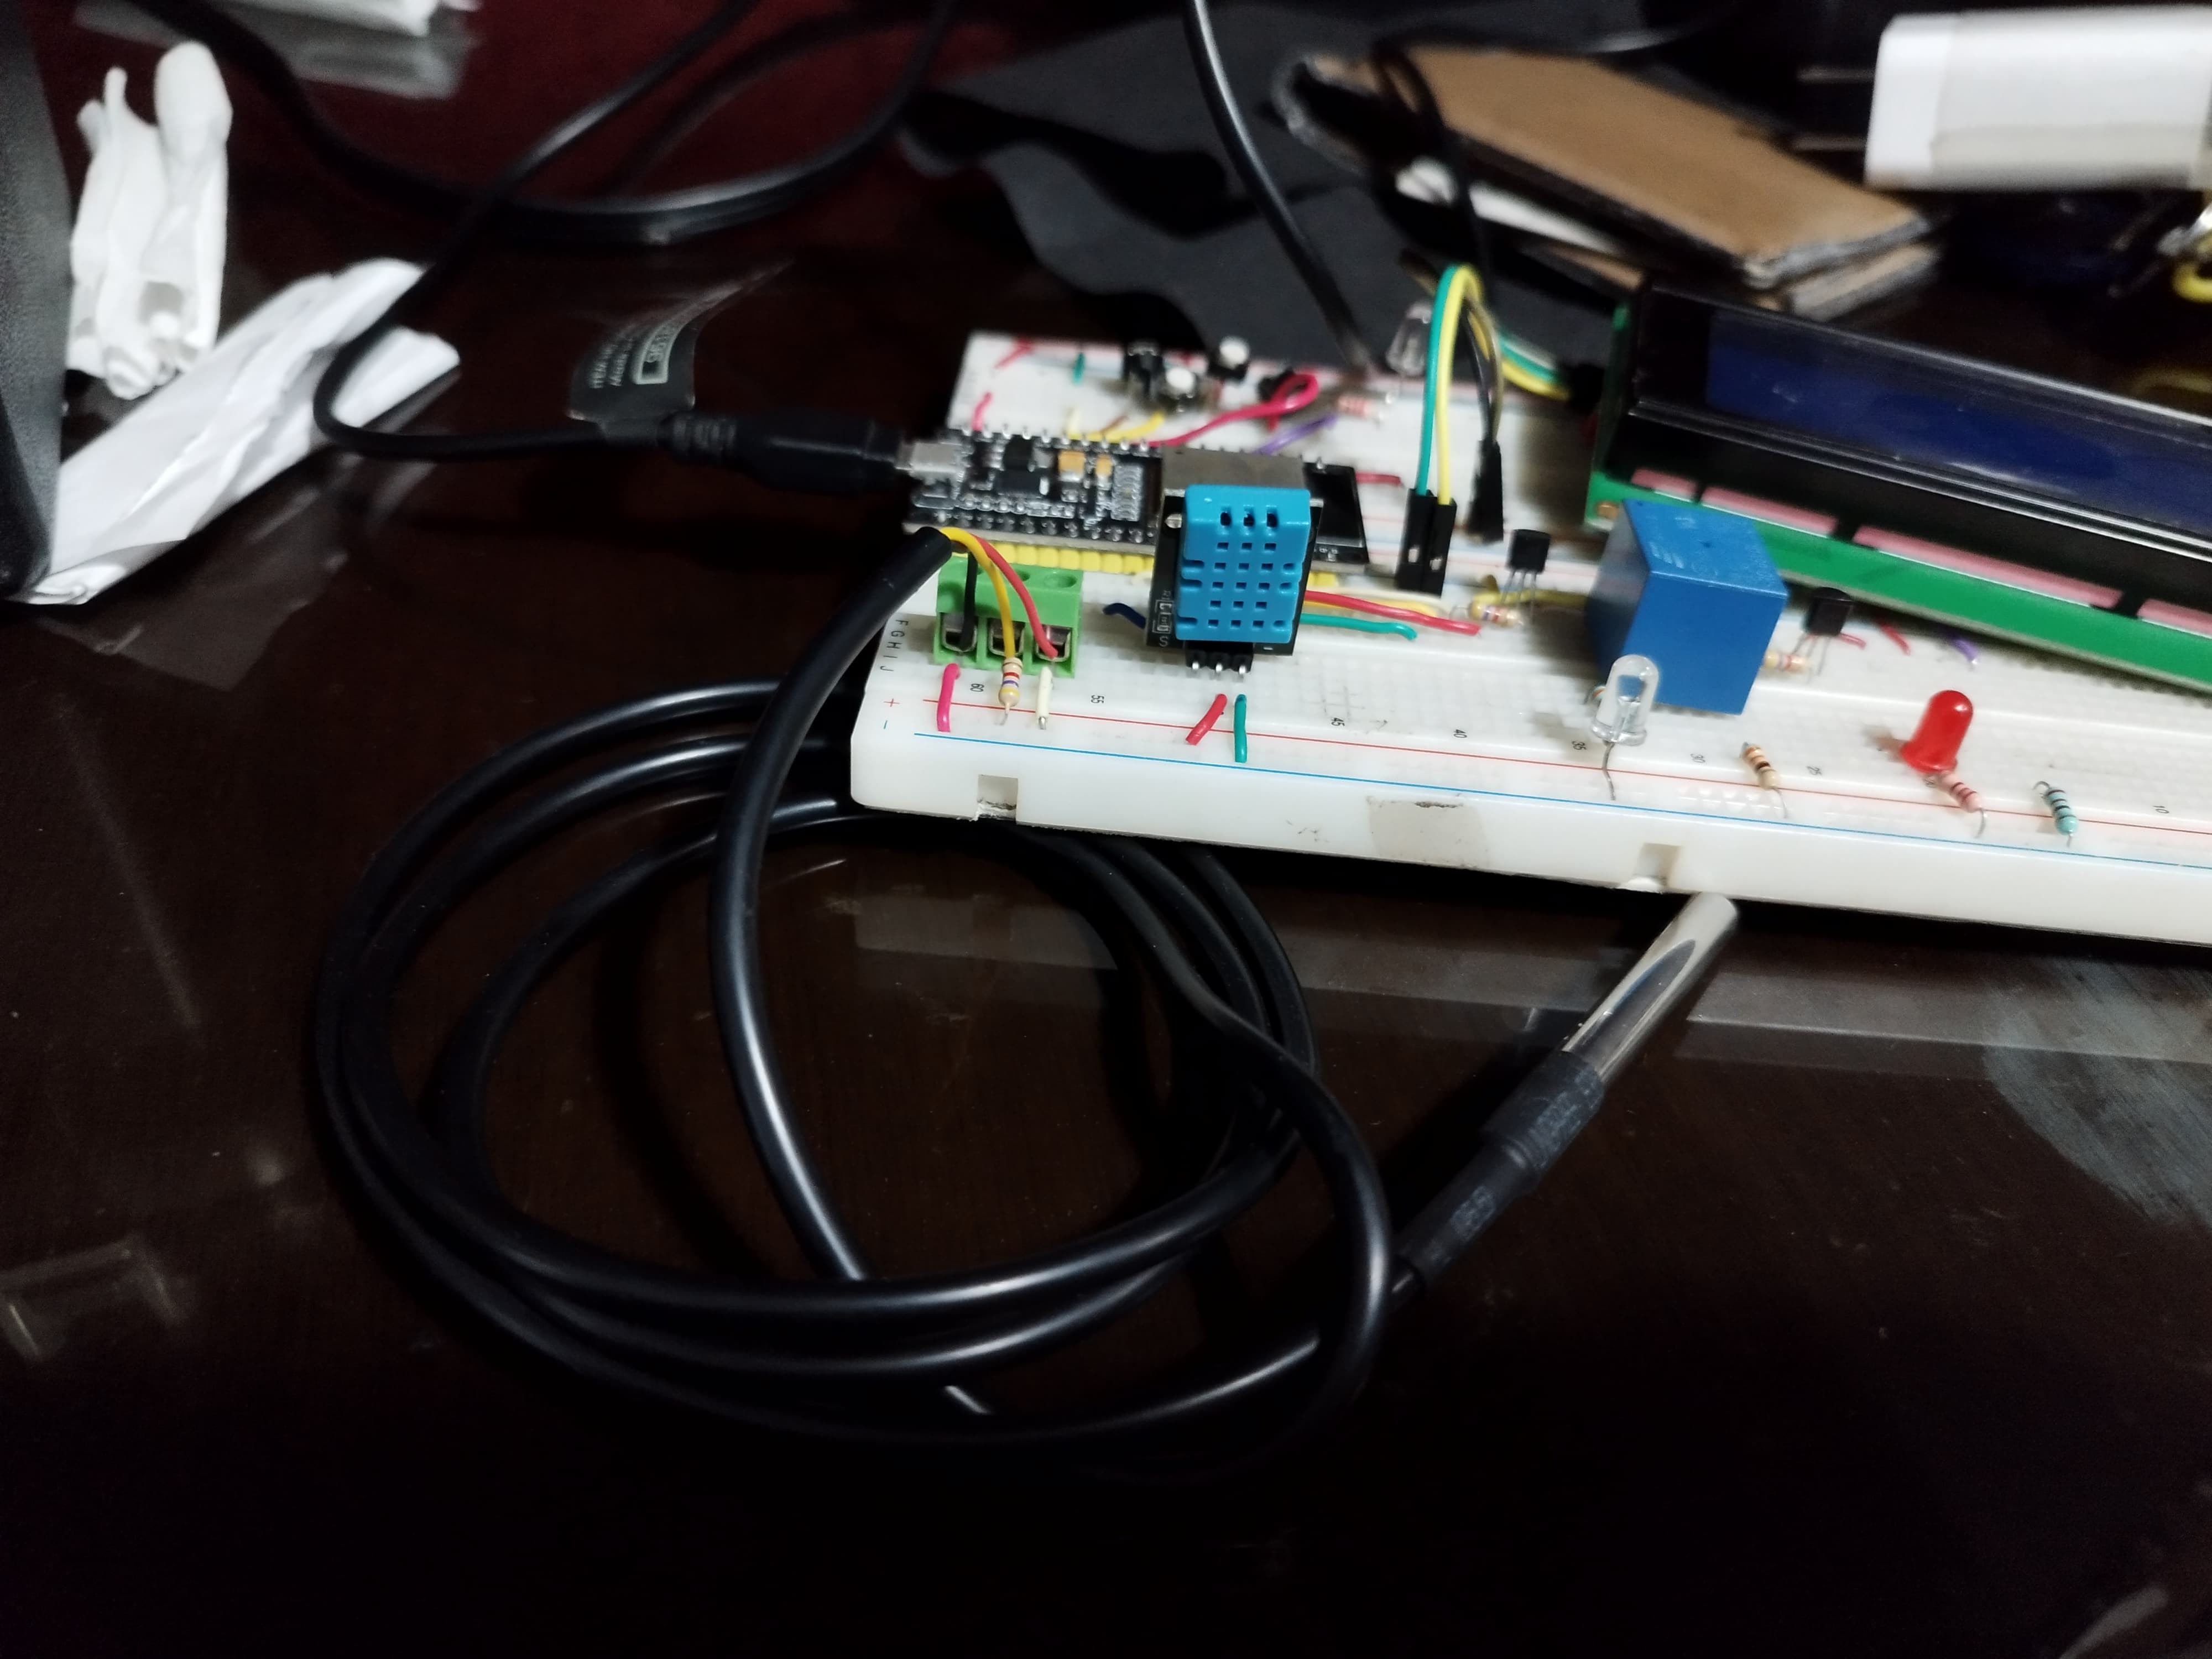
\includegraphics[scale=0.1]{images/Capitulo_Imple/S2/CTO_SEN.jpeg}
            \caption{Conexión de los sensores en la protoboard}
            \label{fg:cto_sensores_impl}
\end{figure}
\clearpage

En caso del sensor DHT11 (figura \ref{fg:DHT11_Fisico}), de humedad, no es necesario realizar alguna conexión externa, debido a que se cuenta con la versión del sensor que viene en una placa PCB, el cual presenta la resistencia de 10 $k\Omega$, por lo que se conecta la señal de lectura, directa al pin 17 de la ESP32.

\begin{figure}[h!]
            \centering
            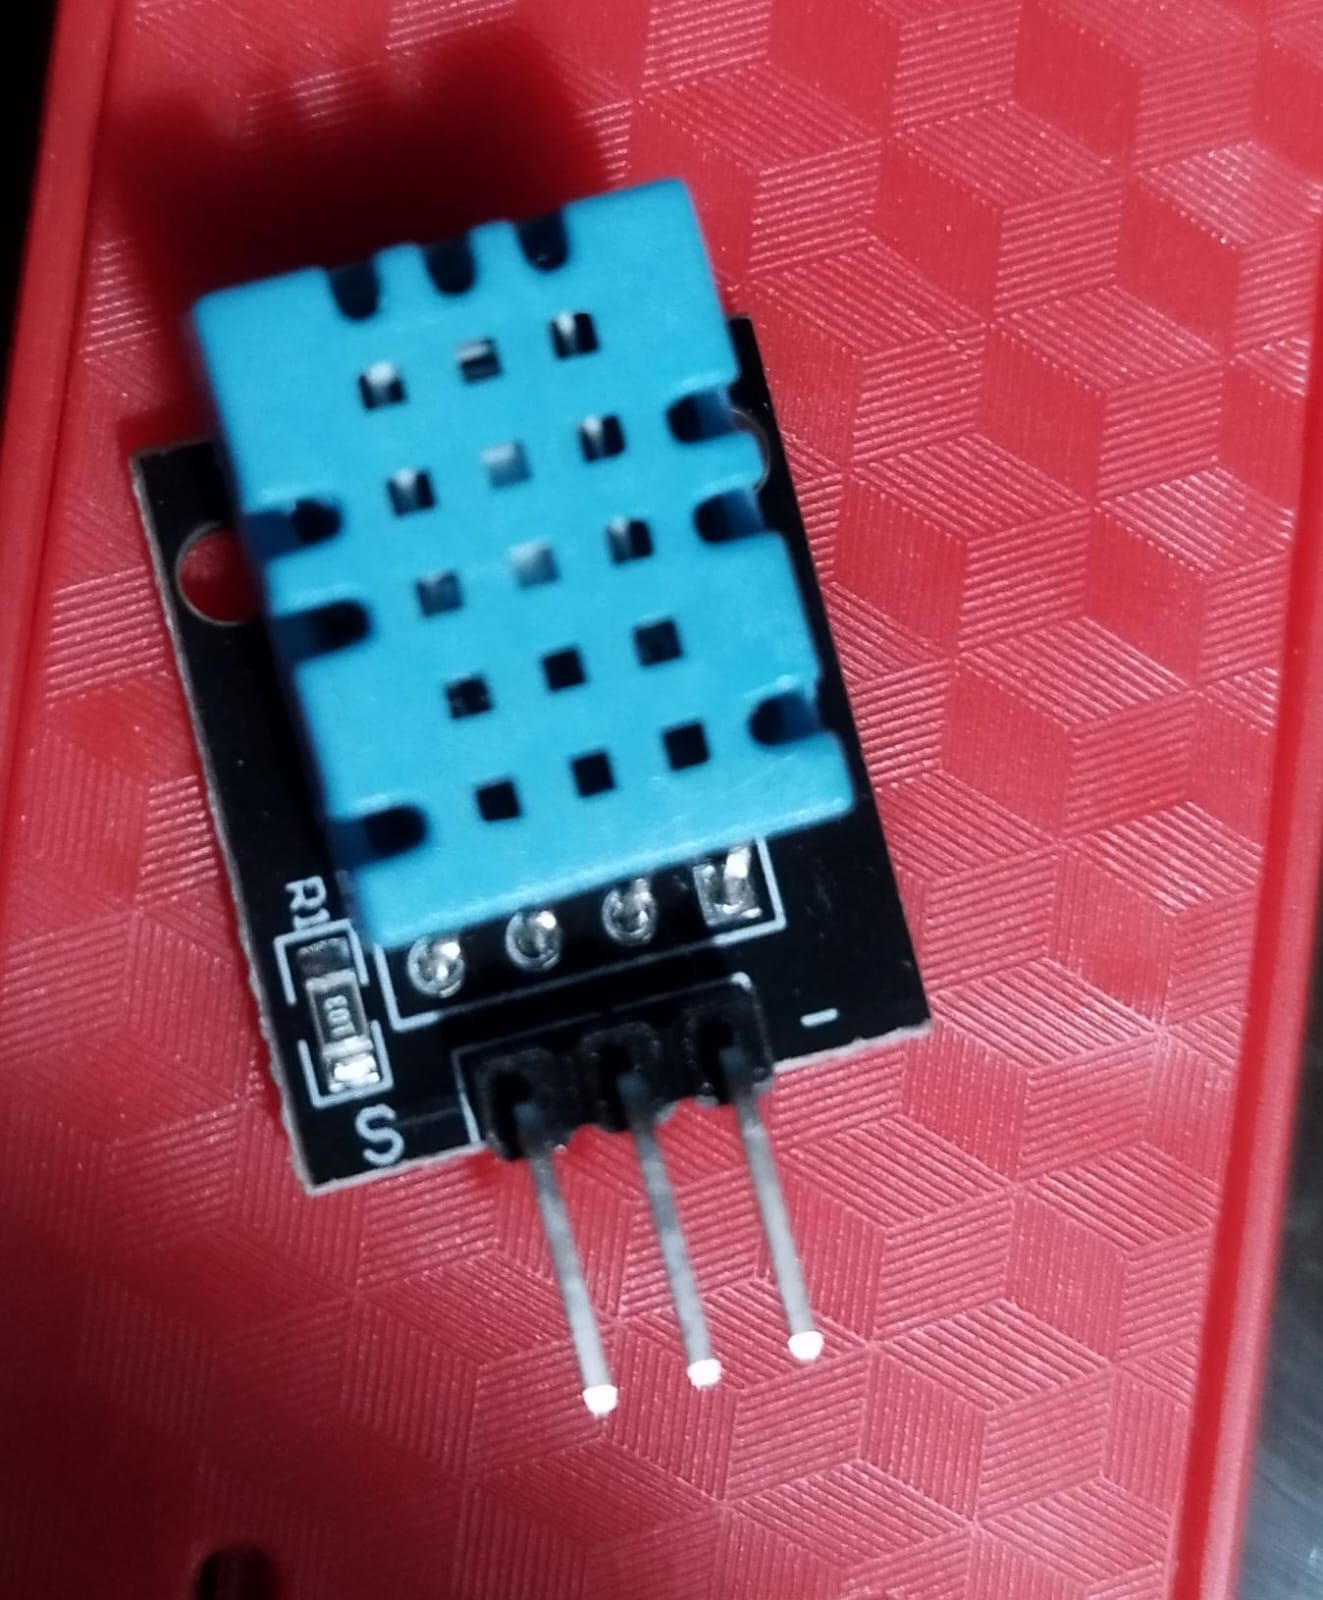
\includegraphics[scale=0.1]{images/Capitulo_Imple/S2/DHT11_FIS.jpeg}
            \caption{Sensor DHT11 que se utilizó}
            \label{fg:DHT11_Fisico}
\end{figure}

Ya conectados, se integran al programa utilizando la biblioteca "DHT sensor library" de Adafruit, "DallasTemperature" de Miles Burton y "OneWire" de Jim Studt para utilizar los acondicionamientos digitales dentro del microprocesador. De esta manera, se leen los valores de las variables físicas y puedan ser mostrados al usuario por medio de la LCD, como se ve en la figura. \ref{fg:cto_senso_funcionando}.

\begin{figure}[h]
            \centering
            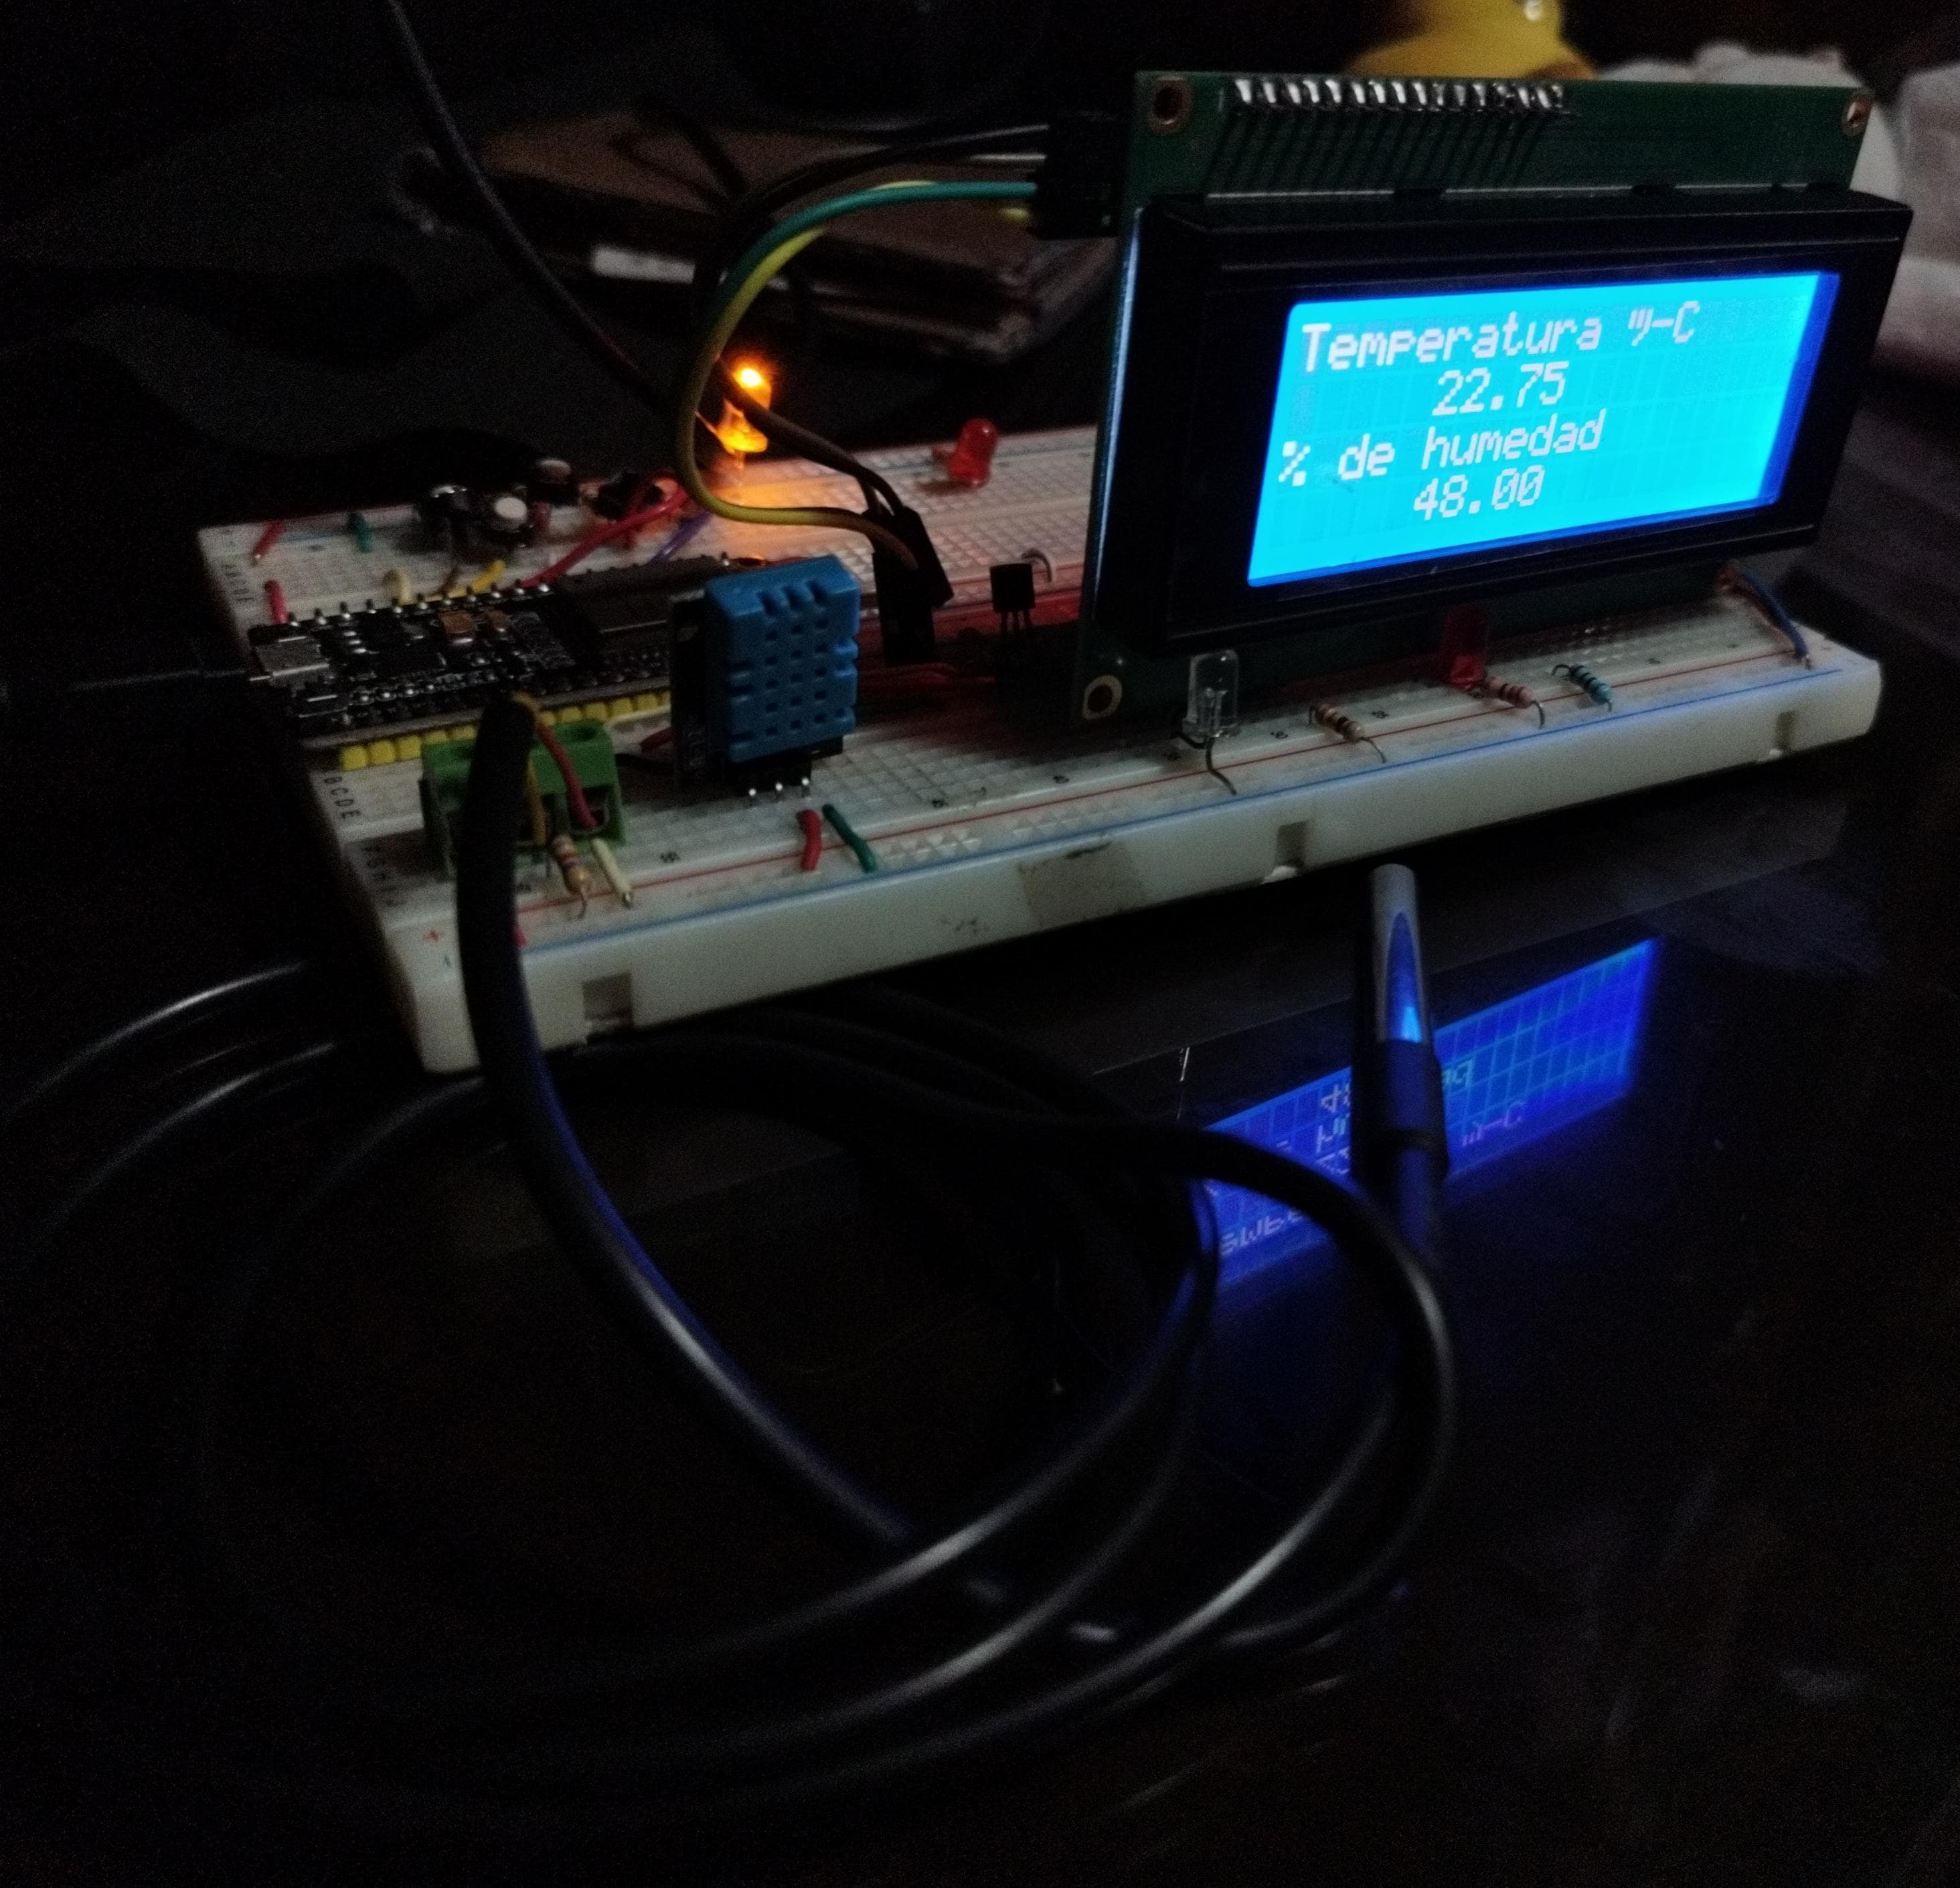
\includegraphics[scale=0.15]{images/Capitulo_Imple/S2/SEN_FUNCIONANDO.jpeg}
            \caption{Circuito de prueba de la interfaz}
            \label{fg:cto_senso_funcionando}
        \end{figure}
\clearpage